%%%%%%%%%%%%%%%%%%%%%%%%%%%%%%%%%%%%%%%%%%%%%%%%%%%%%%%%%%%%%%%%%%%%%%%%%%
%%
%%   IPHIPI -- Agentic AI Mock Interview Platform
%%   Architecture Document
%%
%%   Single-file, vanilla pdflatex, Overleaf-ready.
%%   Compile:  pdflatex ARCHITECTURE.tex   (twice for cross-refs)
%%
%%%%%%%%%%%%%%%%%%%%%%%%%%%%%%%%%%%%%%%%%%%%%%%%%%%%%%%%%%%%%%%%%%%%%%%%%%

\documentclass[11pt,a4paper]{article}

\usepackage[utf8]{inputenc}
\usepackage[T1]{fontenc}
\usepackage[margin=1in,headheight=14pt]{geometry}
\usepackage{xcolor}
\usepackage{hyperref}
\usepackage{booktabs}
\usepackage{tikz}
\usepackage{amsmath}
\usepackage{amssymb}
\usepackage{listings}
\usepackage{enumitem}
\usepackage{titlesec}
\usepackage{fancyhdr}
\usepackage{caption}
\usepackage{array}
\usepackage{lastpage}

\usetikzlibrary{arrows.meta,positioning,shapes,fit,calc,shadows.blur,backgrounds}

%%-------- colours --------%%
\definecolor{brand}{HTML}{5B67FF}
\definecolor{brandDark}{HTML}{2C3289}
\definecolor{accent}{HTML}{8A6BFF}
\definecolor{ink}{HTML}{0A0D18}
\definecolor{paper}{HTML}{FBFBFE}
\definecolor{ruleline}{HTML}{D7D9E4}
\definecolor{tablerow}{HTML}{F2F3F9}
\definecolor{codebg}{HTML}{F4F4F8}
\definecolor{ok}{HTML}{1F8A55}
\definecolor{warn}{HTML}{B5621A}

%%-------- hyperref --------%%
\hypersetup{
  colorlinks=true,
  linkcolor=brandDark,
  urlcolor=brand,
  citecolor=brandDark,
  pdftitle={IPHIPI -- Agentic AI Mock Interview Platform: Architecture},
  pdfauthor={IPHIPI Engineering},
  pdfborder={0 0 0}
}

%%-------- headings --------%%
\titleformat{\section}
  {\Large\bfseries\color{brandDark}}{\thesection}{0.7em}{}
\titleformat{\subsection}
  {\large\bfseries\color{ink}}{\thesubsection}{0.7em}{}
\titleformat{\subsubsection}
  {\normalsize\bfseries\color{ink}}{\thesubsubsection}{0.7em}{}

%%-------- lists --------%%
\setlist[itemize]{leftmargin=1.4em,itemsep=2pt,topsep=2pt}
\setlist[enumerate]{leftmargin=1.6em,itemsep=2pt,topsep=2pt}

%%-------- header / footer --------%%
\pagestyle{fancy}
\fancyhf{}
\renewcommand{\headrulewidth}{0pt}
\fancyhead[L]{\footnotesize\color{black!55}IPHIPI \textbullet\ Architecture}
\fancyhead[R]{\footnotesize\color{black!55}\thepage\ / \pageref{LastPage}}
\fancyfoot[C]{}

%%-------- listings --------%%
\lstdefinelanguage{json}{
  basicstyle=\ttfamily\small,
  numbers=none,
  showstringspaces=false,
  breaklines=true,
  string=[s]{"}{"},
  comment=[l]{//},
  morestring=[b]"
}
\lstset{
  backgroundcolor=\color{codebg},
  basicstyle=\ttfamily\footnotesize,
  frame=single,
  framerule=0pt,
  rulecolor=\color{ruleline},
  framesep=8pt,
  xleftmargin=6pt,
  xrightmargin=6pt,
  breaklines=true,
  showstringspaces=false,
  commentstyle=\color{black!55},
  keywordstyle=\color{brandDark}\bfseries
}

%%-------- TikZ helpers --------%%
\tikzset{
  block/.style={draw=brand!60, rounded corners=4pt, fill=brand!8, minimum width=3.4cm,
                minimum height=1.0cm, font=\sffamily\small, align=center, blur shadow={shadow blur steps=4}},
  store/.style={draw=accent!60, rounded corners=2pt, fill=accent!8, minimum width=2.8cm,
                minimum height=0.9cm, font=\sffamily\footnotesize, align=center},
  ext/.style={draw=ok!60, rounded corners=4pt, fill=ok!8, minimum width=3.0cm,
              minimum height=0.9cm, font=\sffamily\footnotesize, align=center},
  flow/.style={->,>={Stealth[length=2.8mm]}, semithick, draw=ink!60},
  sect/.style={draw=ruleline, dashed, rounded corners=6pt, inner sep=10pt}
}

%%========================================================================%%
\begin{document}

\begin{titlepage}
  \centering
  \vspace*{1cm}
  {\fontsize{32}{36}\selectfont\bfseries\color{brandDark} IPHIPI}\\[0.3em]
  {\Large Agentic AI Mock Interview Platform}\\[2em]
  {\Huge\bfseries Architecture Document}\\[3em]

  
\begin{tikzpicture}
    \node[fill=brand,rounded corners=10pt,minimum width=10cm,minimum height=2.6cm,blur shadow]
      (logo) {};
    \node[white,font=\Large\bfseries] at (logo.center)
      {Six agents. One natural conversation.};
  \end{tikzpicture}

  \vfill
  \begin{tabular}{rl}
    \textbf{Repository}   & \href{https://github.com/roshan5619/Intelligent_Mock_Interview_Agent}
                            {github.com/roshan5619/Intelligent\_Mock\_Interview\_Agent} \\
    \textbf{Live demo}    & \href{https://iphpi-hackthon.vercel.app}{iphpi-hackthon.vercel.app} \\
    \textbf{Document}     & End-to-end design \textbullet\ scoring approach \textbullet\ trade-offs \\
    \textbf{Audience}     & Engineering leadership, hackathon judges, security review \\
    \textbf{Date}         & \today \\
  \end{tabular}
  \vspace{1.2cm}
\end{titlepage}

\tableofcontents
\newpage

%%------------------------------------------------------------------%%
\section{Problem Summary and User Journey}\label{sec:problem}

\subsection{Problem statement}

Senior professionals (10--15+ years of experience) preparing for interviews
suffer from a structural gap in available practice tools:

\begin{itemize}
  \item \textbf{Static question banks} do not adapt to the candidate's resume,
        seniority, or live performance.
  \item \textbf{Generic LLM chats} provide text-only feedback and cannot read
        body language or vocal cues---signals that meaningfully predict
        interview outcomes for senior roles.
  \item \textbf{Scoring is opaque}. Most tools surface a number with no
        evidence and no path to improvement.
\end{itemize}

IPHIPI closes this gap with an \emph{agentic} multimodal platform that:
(i) reads a resume and infers realistic target roles;
(ii) conducts a live video + audio mock interview, dynamically generating
questions and adapting difficulty;
(iii) produces an explainable report with per-dimension scores, evidence
quotes from the transcript, and concrete next steps.

The platform is built entirely on \emph{free} state-of-the-art models
(Groq Llama~3.3~70B, Google Gemini~2.0~Flash, MediaPipe Tasks, Web Audio API)
to remain accessible to individual users.

\subsection{Target user}

The product is calibrated for a senior professional---specifically the brief's
named persona of a 15-year practitioner. This calibration is enforced
throughout the system:
\begin{itemize}
  \item The orchestrator prompt frames the interaction as peer-to-peer,
        not quiz-style.
  \item The technical evaluator's rubric reserves $\geq 0.9$ scores for
        ``genuinely outstanding'' answers; the typical senior answer
        lands in $0.5$--$0.8$.
  \item The agenda planner prefers project deep-dives over fundamentals.
\end{itemize}

\subsection{End-to-end user journey}

\begin{enumerate}
  \item Land on the marketing site (\texttt{/}).
  \item Either browse \texttt{/careers} or upload a resume on
        \texttt{/match-me} for resume-driven role recommendations.
  \item For each open IPHIPI role, the system computes a hybrid match score
        (semantic similarity + weighted skill overlap + seniority fit) with
        an LLM-generated rationale.
  \item Apply to a chosen role $\rightarrow$ candidate page shows the
        animated fit ring, sub-scores, matched skills, and gaps.
  \item Click \emph{Start mock interview} $\rightarrow$ pre-flight requests
        camera + microphone permissions and previews the agenda.
  \item A 30-second warmup loads MediaPipe models, calibrates the
        eye-contact baseline, and the interviewer greets the candidate via
        text-to-speech.
  \item The interview runs hands-free: voice activity detection (VAD)
        auto-starts the candidate's turn $\sim$200~ms after speech begins
        and auto-submits $\sim$900~ms after they stop.
  \item Each turn is scored in parallel by Audio, Visual, and Technical
        agents; the Orchestrator decides the next question and adapts
        difficulty using both LLM judgement and hard heuristics.
  \item End $\rightarrow$ Agent~6 generates a structured report with
        per-dimension scores, quoted evidence, behavioural insights, and
        five concrete next steps.
\end{enumerate}

%%------------------------------------------------------------------%%
\section{High-Level Architecture}\label{sec:arch}

\subsection{Three-tier deployment topology}

\begin{figure}[h]
\centering
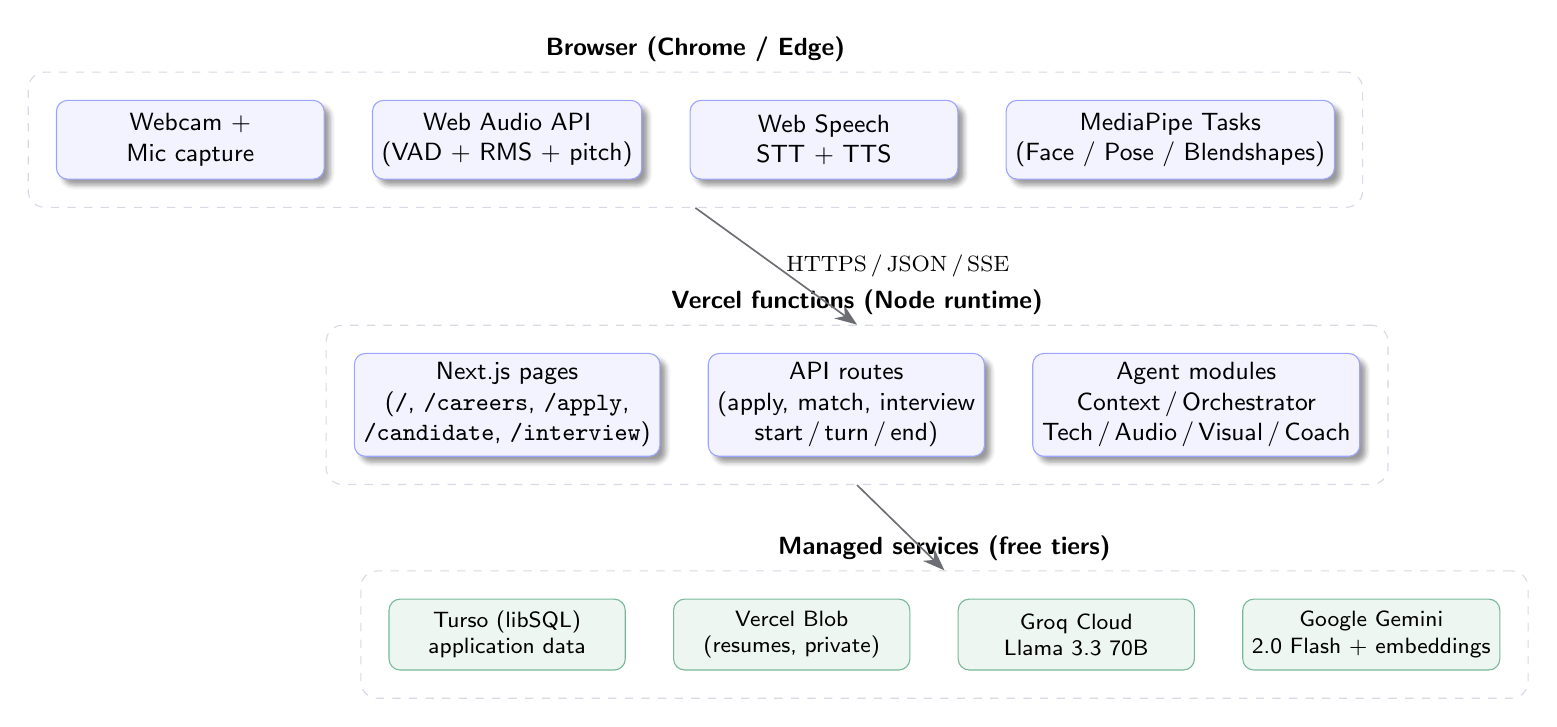
\begin{tikzpicture}[node distance=8mm and 6mm]

  %% Browser tier
  \node[block] (cam)   {Webcam +\\Mic capture};
  \node[block, right=of cam] (audio) {Web Audio API\\(VAD + RMS + pitch)};
  \node[block, right=of audio] (speech) {Web Speech\\STT + TTS};
  \node[block, right=of speech] (mp) {MediaPipe Tasks\\(Face / Pose / Blendshapes)};
  \node[sect, fit=(cam)(audio)(speech)(mp), label={[font=\sffamily\small\bfseries]
        above:Browser (Chrome / Edge)}] (browser) {};

  %% Vercel tier
  \node[block, below=22mm of audio.south] (pages)
        {Next.js pages\\(\texttt{/}, \texttt{/careers}, \texttt{/apply},\\
         \texttt{/candidate}, \texttt{/interview})};
  \node[block, right=of pages] (api)
        {API routes\\(apply, match, interview\\start\,/\,turn\,/\,end)};
  \node[block, right=of api] (agents)
        {Agent modules\\Context\,/\,Orchestrator\\Tech\,/\,Audio\,/\,Visual\,/\,Coach};
  \node[sect, fit=(pages)(api)(agents), label={[font=\sffamily\small\bfseries]
        above:Vercel functions (Node runtime)}] (vercel) {};

  %% External tier
  \node[ext, below=18mm of pages.south] (turso) {Turso (libSQL)\\application data};
  \node[ext, right=of turso] (blob) {Vercel Blob\\(resumes, private)};
  \node[ext, right=of blob] (groq) {Groq Cloud\\Llama 3.3 70B};
  \node[ext, right=of groq] (gemini) {Google Gemini\\2.0 Flash + embeddings};
  \node[sect, fit=(turso)(blob)(groq)(gemini), label={[font=\sffamily\small\bfseries]
        above:Managed services (free tiers)}] (svc) {};

  %% Flows
  \draw[flow] (browser.south) -- node[right,font=\footnotesize]{HTTPS\,/\,JSON\,/\,SSE} (vercel.north);
  \draw[flow] (vercel.south) -- (svc.north);

\end{tikzpicture}
\caption{Three-tier deployment topology. Raw video and audio never leave the
browser; only $\sim$2 KB of aggregated metric JSON is sent per turn.}
\end{figure}

\subsection{Module / agent inventory}

\begin{table}[h]
\centering
\renewcommand{\arraystretch}{1.25}
\begin{tabular}{@{}p{0.6cm} p{4.0cm} p{2.5cm} p{6.5cm}@{}}
\toprule
\textbf{\#} & \textbf{Agent} & \textbf{Runs in} & \textbf{Backing technology} \\
\midrule
1 & Context Understanding   & Server         & Gemini 2.0 Flash (native PDF) $+$ Groq fallback \\
2 & Interview Orchestrator  & Server         & Groq Llama 3.3 70B + adaptive heuristics \\
3 & Audio Intelligence      & Browser$+$Server & Web Audio API capture; Groq scoring \\
4 & Visual Intelligence     & Browser only   & MediaPipe FaceLandmarker, PoseLandmarker, Blendshapes (pretrained, no LLM) \\
5 & Technical Evaluation    & Server         & Groq Llama 3.3 70B with concept-coverage rubric \\
6 & Feedback \& Coaching    & Server         & Groq Llama 3.3 70B aggregating all per-turn signals \\
\bottomrule
\end{tabular}
\caption{The six-agent inventory.}
\end{table}

\subsection{Per-turn data flow}

\begin{figure}[h]
\centering
\begin{tikzpicture}[
  node distance=4mm and 18mm,
  step/.style={draw=ink!40, rounded corners=3pt, fill=paper, font=\sffamily\footnotesize, minimum width=3.3cm, minimum height=0.9cm, align=center},
  para/.style={draw=brand!60, fill=brand!8, rounded corners=3pt, font=\sffamily\footnotesize\bfseries, minimum width=3.3cm, minimum height=0.9cm, align=center}
  ]
  \node[step] (s1) {Browser flushes\\AudioMetrics + VisualMetrics};
  \node[step, below=of s1] (s2) {POST \texttt{/api/interview/turn}};
  \node[step, below=of s2] (s3) {Persist candidate turn};

  \node[para, right=22mm of s3] (a3) {Agent 3 (audio LLM)};
  \node[para, below=2mm of a3] (a4) {Agent 4 (visual deterministic)};
  \node[para, below=2mm of a4] (a5) {Agent 5 (technical LLM)};

  \node[step, below=12mm of s3] (s4) {Persist all per-dimension\\\texttt{agent\_evaluations} rows};
  \node[step, below=of s4] (s5) {Build 2-turn confidence\\and correctness trends};
  \node[step, below=of s5] (s6) {Agent 2 (Orchestrator) decides next turn\\\emph{adaptive heuristics may override}};
  \node[step, below=of s6] (s7) {Persist new agent turn $+$ return JSON};
  \node[step, below=of s7] (s8) {Browser speaks question via TTS\\$\rightarrow$ listening (loop)};

  \draw[flow] (s1)--(s2);
  \draw[flow] (s2)--(s3);
  \draw[flow] (s3.east) -| ([xshift=-6mm]a3.west) -- (a3.west);
  \draw[flow] (s3.east) -| ([xshift=-6mm]a4.west) -- (a4.west);
  \draw[flow] (s3.east) -| ([xshift=-6mm]a5.west) -- (a5.west);
  \draw[flow] (a3.south west) ..controls +(-1.4,-0.5) and +(1.4,0.5).. (s4.east);
  \draw[flow] (a4.south west) ..controls +(-1.4,-0.5) and +(1.4,0.5).. (s4.east);
  \draw[flow] (a5.south west) ..controls +(-1.4,-0.5) and +(1.4,0.5).. (s4.east);
  \draw[flow] (s4)--(s5);
  \draw[flow] (s5)--(s6);
  \draw[flow] (s6)--(s7);
  \draw[flow] (s7)--(s8);
  \draw[flow] (s8.south) ..controls +(-3.5,-0.5) and +(-3.5,3.0).. (s1.west);
\end{tikzpicture}
\caption{One interview turn. The three evaluators (Agents 3, 4, 5) run in
parallel via \texttt{Promise.all}; Agent 2 only fires after their results
are persisted, so it can read 2-turn trends.}
\end{figure}

\subsection{Interfaces}

The system exposes four production HTTP interfaces. All accept JSON or
\texttt{multipart/form-data} and run on the Node runtime with
\texttt{maxDuration = 60} seconds.

\begin{table}[h]
\centering
\renewcommand{\arraystretch}{1.25}
\begin{tabular}{@{}p{4.6cm} p{4.0cm} p{6.4cm}@{}}
\toprule
\textbf{Endpoint} & \textbf{Method / body} & \textbf{Function} \\
\midrule
\texttt{/api/apply}                    & POST multipart  & Resume upload, Agent 1, JD match for one job, persist application \\
\texttt{/api/match/rank-all}           & POST multipart  & Resume upload, Agent 1, score against all IPHIPI jobs, persist run \\
\texttt{/api/interview/start}          & POST JSON       & Build agenda, create session, run Orchestrator opening turn \\
\texttt{/api/interview/turn}           & POST JSON       & Persist candidate turn $\rightarrow$ parallel Agents 3/4/5 $\rightarrow$ Agent 2 next turn \\
\texttt{/api/interview/end}            & POST JSON       & Run Agent 6 over transcript, persist report \\
\texttt{/api/health}                   & GET             & Diagnostic: env-var presence + live DB connectivity \\
\bottomrule
\end{tabular}
\caption{Production HTTP interfaces.}
\end{table}

The internal LLM interface is a single typed router (\texttt{lib/llm/client.ts})
exposing \texttt{generate}, \texttt{generateStream}, \texttt{generateFromPdf},
and \texttt{embed}---each one falling back through the chain
$\text{Groq} \rightarrow \text{Gemini} \rightarrow \text{Ollama}$ if a
provider is rate-limited or unavailable.

%%------------------------------------------------------------------%%
\section{Key Design Choices and Trade-offs}\label{sec:choices}

\subsection{Browser-side multimodal capture and ML}

\paragraph{Decision.} All webcam frames, microphone samples, voice activity
detection, speech-to-text, text-to-speech, and computer-vision inference
run client-side in the browser. Only $\sim$2 KB of aggregated metric
JSON is transmitted per turn.

\paragraph{Trade-off considered.}
A server-side pipeline using OpenCV/MediaPipe-on-GPU would give us identical
signals with better baseline performance on cheap clients. We rejected it
because (i) it requires shipping raw video over the wire, raising privacy
and bandwidth costs; (ii) it would require GPU-backed Vercel functions,
ending the free-tier story; (iii) the brief explicitly asked us to
\emph{prefer pretrained CV over LLMs}, which MediaPipe Tasks (WASM,
free, $\sim$15--30 FPS in-browser) satisfies natively.

\paragraph{Result.} Privacy is provable from the network tab: the user can
verify that no video buffer ever leaves their device. Latency is the
sum of one model call per turn (the Orchestrator), not the round-trip
of multiple multi-megabyte video frames.

\subsection{Multi-provider LLM router with auto-fallback}

The router (Listing~\ref{lst:router}) accepts a single typed request and
walks a fallback chain. Each provider self-reports availability based
on the presence of its API key; none of the agents see provider-specific
SDKs.

\begin{lstlisting}[language=json,caption={Router fallback order.},label={lst:router}]
preferred provider (per-agent config) ->  Groq Llama 3.3 70B
                                      ->  Google Gemini 2.0 Flash
                                      ->  Local Ollama (offline only)
\end{lstlisting}

\paragraph{Why Groq is primary.} Three reasons.
\begin{enumerate}
  \item \emph{Speed.} Groq's hosted Llama 3.3 70B runs at $\sim$500 tokens
        per second. The Orchestrator first-token latency drops to
        $\sim$300~ms. This is the difference between an interview that
        feels alive and one that feels sluggish.
  \item \emph{Quality.} Llama 3.3 70B is near-frontier on general reasoning
        benchmarks. We do not need GPT-4-class quality for question
        generation or rubric scoring.
  \item \emph{Cost.} Free tier of 30~RPM and 14{,}400~RPD covers a typical
        demo and early users.
\end{enumerate}

\paragraph{Why Gemini for PDFs.} Gemini 2.0 Flash natively understands PDF
bytes. We pass the inline base64 PDF together with the system prompt; no
\texttt{pdf-parse} step is required for the happy path. The
\texttt{text-extraction $\rightarrow$ Groq} fallback only fires when
Gemini is rate-limited.

\subsection{Single base model, six system prompts}

All server-side agents target the same base model
(Llama 3.3 70B on Groq). We tune \texttt{temperature}, \texttt{top\_p},
and \texttt{response\_format} per agent (Table~\ref{tab:per-agent}), but
we do not swap models per agent.

\begin{table}[h]
\centering
\renewcommand{\arraystretch}{1.25}
\begin{tabular}{@{}lrrl@{}}
\toprule
\textbf{Agent} & \textbf{temp.} & \textbf{top\_p} & \textbf{response} \\
\midrule
Context Understanding   & 0.20 & 1.00 & JSON  \\
Orchestrator            & 0.70 & 0.90 & JSON  \\
Audio Intelligence      & 0.10 & 1.00 & JSON  \\
Technical Evaluation    & 0.20 & 1.00 & JSON  \\
JD-match rationale      & 0.40 & 1.00 & text  \\
Feedback \& Coaching    & 0.60 & 1.00 & JSON  \\
\bottomrule
\end{tabular}
\caption{Per-agent sampling configuration. Source:
\texttt{lib/llm/config.ts}.}\label{tab:per-agent}
\end{table}

\paragraph{Why not a different model per agent?} Operationally, one model
gives one latency profile, one cost profile, and one set of failure modes
to characterise. The marginal quality from picking a specialist model per
task (e.g., a coding-tuned model for technical eval) is dominated by the
quality of the system prompt and the temperature setting.

\subsection{Async non-blocking evaluators}

The three per-turn evaluators (Agents 3, 4, 5) execute in parallel via
\texttt{Promise.all}. Agent 4 is pure deterministic math and returns
synchronously; Agents 3 and 5 are independent LLM calls.

The candidate-perceived latency per turn is therefore:
\begin{equation}
T_{\text{turn}} \approx \max\!\bigl(T_3,\,T_4,\,T_5\bigr) \;+\; T_2
\;\approx\; 1.0\text{--}1.5\,\text{s} \;+\; 1.0\text{--}1.5\,\text{s}
\end{equation}
yielding $\sim$2--3~s end-to-end. With sequential execution this would
be $\sim$5--6~s, which is conversationally awkward.

\subsection{Adaptive difficulty as code, not prompt}

The Orchestrator's system prompt instructs the LLM to consider the
candidate's confidence and correctness trends. We do \emph{not} trust
this alone. Three hard heuristics layer on top of the LLM's decision
(Listing~\ref{lst:heuristics}) and override the intent if needed.

\begin{lstlisting}[language=json,caption={Adaptive difficulty heuristics
applied server-side after the LLM call.},label={lst:heuristics}]
if confidence_trend has 2 consecutive turns < 0.4
   -> intent := drop_difficulty
   -> prepend warm encouragement to the question

if correctness_trend has 2 consecutive turns > 0.85
   -> intent := ramp_difficulty

if time_budget_remaining < 2 minutes
   -> intent := wrap_up
\end{lstlisting}

The LLM still writes the actual sentence; the policy is code.

\subsection{No authentication in the prototype}

Candidate identity is stored in a signed cookie:
\[
\text{cookie} = \mathrm{base64url}(\text{payload})\,.\,\mathrm{base64url}\bigl(\text{HMAC-SHA256}_{K}(\text{payload})\bigr)
\]
where $K$ is \texttt{HMAC\_SECRET}. Every protected route verifies that
the cookie's candidate ID matches the application or session being acted
on. Magic-link authentication via Supabase is queued for v2.

\subsection{Storage choices}

\begin{table}[h]
\centering
\renewcommand{\arraystretch}{1.25}
\begin{tabular}{@{}p{3.0cm} p{4.6cm} p{7.2cm}@{}}
\toprule
\textbf{Domain} & \textbf{Service} & \textbf{Reason} \\
\midrule
Application data & Turso (libSQL)        & SQLite-compatible managed DB; same DAL works on Postgres in v2; local dev falls back to a SQLite file. \\
Resume PDFs      & Vercel Blob (private) & 1 GB free tier; \texttt{access:'private'}; downloads server-side via \texttt{head()} signed URLs. \\
Secrets          & Vercel Env Vars       & Per-environment (Production / Preview / Development); never in client bundles. \\
\bottomrule
\end{tabular}
\caption{Storage and configuration choices.}
\end{table}

%%------------------------------------------------------------------%%
\section{Scoring Approach}\label{sec:scoring}

The platform produces five families of scores: a one-shot \emph{JD match}
score on apply, and four per-turn evaluator outputs (audio, visual,
technical) plus the final aggregated report.

\subsection{JD match score (apply / match-me)}

For a candidate profile $P$ and a job $J$, we compute a hybrid score
in $[0, 100]$:
\begin{equation}
\mathrm{score}(P, J) = \bigl(0.4 \cdot s_{\text{emb}} + 0.4 \cdot s_{\text{skill}} + 0.2 \cdot s_{\text{senior}}\bigr) \cdot 100
\end{equation}

\paragraph{Embedding similarity.} We embed a textual rendering of the
profile (skills, domains, role titles, project summaries, seniority
signals) and the job (title, level, must-haves, responsibilities) using
\texttt{gemini-embedding-001} (768-dimensional), then compute cosine
similarity:
\begin{equation}
s_{\text{emb}} = \mathrm{clamp}\!\left(\frac{\mathbf{e}_P \cdot \mathbf{e}_J}{\lVert \mathbf{e}_P \rVert\,\lVert \mathbf{e}_J \rVert},\; 0,\; 1\right)
\end{equation}

\paragraph{Weighted skill overlap.} Each requirement in the JD has a
weight ($w_{\text{must}} = 1.0$ for must-haves; $w_{\text{nice}} = 0.4$
for nice-to-haves). For each requirement~$r$:
\begin{equation}
\mathrm{matched}(r, P) = \begin{cases}
1 & \text{if any content word of } r \text{ appears in } P\text{'s tokens} \\
0 & \text{otherwise}
\end{cases}
\end{equation}
\begin{equation}
s_{\text{skill}} = \frac{\sum_{r \in R} w_r \cdot \mathrm{matched}(r, P)}{\sum_{r \in R} w_r}
\end{equation}

\paragraph{Seniority fit.} Given $y_{\text{cand}}$ years total and the
job's $[\,y_{\min}, y_{\max}\,]$ window:
\begin{equation}
s_{\text{senior}} = \begin{cases}
1.0 & y_{\min} \le y_{\text{cand}} \le y_{\max} \\
0.7 & y_{\min}-2 \le y_{\text{cand}} \le y_{\max}+4 \\
0.4 & y_{\text{cand}} \ge y_{\min}-4 \\
0.1 & \text{otherwise}
\end{cases}
\end{equation}

\paragraph{Rationale generation.} After the deterministic numeric scoring,
the LLM is asked to produce a 2--3 sentence ``why this fits'' rationale
\emph{grounded in the matched / gap lists}, never overriding the score.

\subsection{Audio scoring (Agent 3)}

\paragraph{Browser-side signal extraction.} The \texttt{AudioAnalyzer}
samples the microphone at 50~ms intervals and computes per-turn:

\begin{itemize}
  \item RMS mean and variance (volume envelope)
  \item Pitch mean $F_0$ and variance via time-domain autocorrelation
  \item Pause ratio: number of silences $\geq 500$~ms divided by turn duration
  \item Silence percentage: fraction of windows below the silence threshold
  \item Words per minute (WPM) from the live transcript
  \item Filler-word rate (\texttt{um, uh, like, you know}) per minute
\end{itemize}

\paragraph{Voice activity detection.} A two-state machine on RMS samples
gates the conversation:
\begin{itemize}
  \item NOT\_SPEAKING $\rightarrow$ SPEAKING when RMS exceeds $0.030$ for
        $\geq 200$~ms (sustained speech).
  \item SPEAKING $\rightarrow$ NOT\_SPEAKING when RMS stays below $0.030$
        for $\geq 900$~ms (sustained silence).
\end{itemize}
The latter triggers automatic submission of the candidate's turn.

\paragraph{Server-side scoring.} The Audio agent (Groq Llama 3.3 70B,
JSON mode, temperature 0.1) ingests the metric blob and the transcript
and returns:
\begin{lstlisting}[language=json]
{
  "confidence": 0..1,
  "clarity":    0..1,
  "evidence":         "1 sentence quoting a real signal",
  "signals_summary":  "1 sentence interpretation"
}
\end{lstlisting}

\paragraph{Rubric anchors.}
\begin{itemize}
  \item Confidence is HIGH ($>0.7$) when WPM is in $[110, 160]$, fillers
        $<2$/min, pitch variance is healthy, and silence percentage $<0.2$.
  \item Confidence is LOW ($<0.4$) when WPM is erratic OR fillers $>6$/min
        OR pitch is very flat OR silence percentage $>0.4$.
  \item Clarity rewards visible structure (problem $\rightarrow$ approach
        $\rightarrow$ outcome; STAR for behavioural).
\end{itemize}

\subsection{Visual scoring (Agent 4)}

\paragraph{Browser-side metrics.} MediaPipe \texttt{FaceLandmarker} (478
landmarks, 52 blendshapes) and \texttt{PoseLandmarker} (33 keypoints) run
at $\sim$15~FPS. The \texttt{VisionMetricsAggregator} per-turn output:

\begin{itemize}
  \item \texttt{eye\_contact\_ratio}: fraction of frames where the nose
        tip is centred AND within $\pm 0.08$ normalized units of the
        eye-contact baseline calibrated during the warmup.
  \item \texttt{head\_pose\_stability}: $1 - \alpha (\sigma_x^2 + \sigma_y^2)$
        of the nose tip across the turn.
  \item \texttt{posture\_score}: shoulder-Y symmetry combined with
        head-over-shoulder centring.
  \item Smile, brow-raise, jaw-tension blendshape means.
  \item Blink rate per minute.
\end{itemize}

\paragraph{Deterministic server scoring.} Per the brief's preference for
pretrained CV over LLMs, the server applies fixed formulas (no model call):
\begin{align}
\mathrm{engagement} &= 0.5 + 0.25\,(e - 0.5) + 0.15\,(s + b) + 0.10\,(h - 0.5) \\
\mathrm{stress}     &= 0.5\,j + 0.3\,(1 - e) + 0.2\,(1 - h)
\end{align}
where $e = \texttt{eye\_contact\_ratio}$, $s = \texttt{smile}$, $b =
\texttt{brow\_raise}$, $h = \texttt{head\_pose\_stability}$, $j =
\texttt{jaw\_tension}$. Both are clamped to $[0, 1]$.

\subsection{Technical scoring (Agent 5)}

The Technical Evaluation agent (Groq, JSON mode, temperature 0.2) scores
each candidate answer against the question that triggered it.

\begin{lstlisting}[language=json]
{
  "correctness":      0..1,  // technical accuracy of the claims
  "depth":            0..1,  // tradeoffs, edge cases, alternatives
  "specificity":      0..1,  // numbers, named systems, observed outcomes
  "concept_coverage": 0..1,  // expected concepts touched / total
  "evidence_quote":   "MUST be a substring of the candidate's answer",
  "flags":            ["hallucination" | "contradiction_with_resume"
                     | "off_topic" | "insufficient_detail"]
}
\end{lstlisting}

The prompt explicitly anchors calibration: ``most senior-engineer answers
fall in 0.5--0.8; reserve 0.9+ for genuinely outstanding answers.'' This
prevents score inflation, which is a known LLM-as-judge failure mode.

\subsection{Aggregation into the final report (Agent 6)}

At end of session, Agent 6 reads the full transcript and every
\texttt{agent\_evaluations} row. It computes per-dimension averages and
identifies the most extreme moments:

\begin{itemize}
  \item Low-confidence moments: turns with confidence $< 0.4$.
  \item Stress peaks: turns with stress $> 0.7$.
\end{itemize}

The LLM produces five sections: \texttt{summary\_md},
\texttt{strengths\_md}, \texttt{improvements\_md},
\texttt{behavioral\_insights\_md}, \texttt{next\_steps\_md}, plus four
0--100 dimension scores. The final \emph{overall} score is recomputed
server-side using the weighted formula:
\begin{equation}
\mathrm{overall} = 0.35 \cdot \tau + 0.30 \cdot \kappa + 0.20 \cdot \gamma + 0.15 \cdot \eta
\end{equation}
where $\tau, \kappa, \gamma, \eta \in [0, 100]$ are the technical,
communication, confidence, and engagement scores respectively. Recomputing
server-side prevents the LLM from drifting on the weighting.

\subsection{Why every score must ship with evidence}

A core design rule: every per-turn evaluation includes either
\texttt{evidence\_quote} (substring of the answer) or
\texttt{signals\_summary} (interpretation of the metrics); every report
bullet quotes a moment from the transcript. ``You scored 71'' is useless
to a senior candidate; ``You scored 71 because in turn 4 you led with
the technology stack rather than the constraint it solved'' is actionable.

%%------------------------------------------------------------------%%
\section{Limitations, Assumptions, and Next Steps}\label{sec:future}

\subsection{Limitations}

\begin{description}[style=nextline]
  \item[Browser support.] The Web Speech API and MediaPipe Tasks both
        require a Chromium-based browser. Firefox lacks \texttt{SpeechRecognition}
        entirely. The ``Type instead'' toggle is the universal fallback.
  \item[Concurrency.] Groq's free tier is capped at 30 requests per
        minute. Sustained concurrent interviews would saturate it; the
        provider router falls back to Gemini, but Gemini's free tier is
        smaller still. A paid tier or a queue is required for production
        scale.
  \item[Resume formats.] Only PDF is supported. \texttt{.docx} or
        \texttt{.txt} would require additional parsing logic, though
        Gemini's PDF understanding handles every PDF variant we have
        tested (column layouts, embedded fonts, scanned PDFs with OCR).
  \item[Single language.] Prompts and STT default to English. Multilingual
        support is a v2 swap (Gemini supports many languages natively;
        Web Speech is locale-dependent).
  \item[No real-time interruption.] The candidate must finish their turn
        before the next interviewer turn fires. Real interruption (the
        candidate cutting off the AI) would require a duplex audio
        channel.
  \item[VAD sensitivity.] In a noisy environment, the voice-activity
        detector can false-trigger. The user can switch to text mode at
        any time; we do not currently auto-detect noise floor.
  \item[Vision baseline.] Eye contact is approximated from head pose,
        not iris gaze. This is sufficient for ``is the candidate facing
        the camera'' but cannot distinguish between looking at notes
        on the screen versus looking at the interviewer pane.
\end{description}

\subsection{Assumptions}

\begin{itemize}
  \item Candidate has a webcam, a microphone, decent lighting, and a
        quiet environment.
  \item Modern Chromium-based browser (Chrome, Edge, Brave).
  \item English fluency.
  \item LLM providers reachable from the Vercel deployment region.
  \item Resume content is the candidate's own (we do not detect plagiarism
        or fabricated experience beyond Agent 5's
        \texttt{contradiction\_with\_resume} flag during the interview).
\end{itemize}

\subsection{Next steps (v2 roadmap)}

\begin{enumerate}
  \item \textbf{Authentication.} Replace the HMAC cookie with Supabase
        magic-link auth. Add a returning-candidate dashboard with
        interview history.
  \item \textbf{Voice quality.} Swap Web Speech for Deepgram (STT) and
        ElevenLabs (TTS). Cross-browser, broadcast quality.
  \item \textbf{Higher-quality reasoning.} Add Anthropic Claude Sonnet
        4.6 as a third provider; route the Feedback agent there for
        report-quality wins on long context.
  \item \textbf{Evaluation harness.} Golden interview transcripts plus
        LLM-as-judge regression tests on every prompt change. Block
        merges that drop scores by more than $\Delta$.
  \item \textbf{Audit log.} Persist every agent decision (orchestrator
        intent, technical eval flags, score) to a separate
        \texttt{agent\_decisions} table for compliance review.
  \item \textbf{Multi-tenant scaling.} Upstash Redis token-bucket rate
        limiting per user and per IP. Warm-pool pre-allocated Vercel
        functions per region.
  \item \textbf{ATS integration.} For paid customers, push the
        \texttt{ContextProfile} and report scores into Greenhouse,
        Lever, and Workday via their public APIs.
  \item \textbf{Real-time interruption.} Move from request/response to a
        WebSocket or WebRTC duplex audio channel so the candidate can
        cut off the interviewer naturally.
  \item \textbf{Mobile.} The interview workspace currently targets
        desktop. A mobile-friendly layout with a smaller webcam and
        a swipeable agenda is the next UI track.
  \item \textbf{Compliance.} GDPR consent at upload, 30-day retention
        with auto-deletion, an opt-out path for using transcripts as
        training data, and an explicit data-processing addendum for
        enterprise customers.
\end{enumerate}

%%------------------------------------------------------------------%%
\section{Running the Project Locally}\label{sec:run}

\subsection{Prerequisites}

\begin{itemize}
  \item \textbf{Node.js} 20 LTS or newer (\texttt{node -{}-version} should
        report \texttt{v20.x} or higher).
  \item \textbf{Git} (any recent version).
  \item A \textbf{Chromium-based browser} (Chrome / Edge / Brave) for the
        interview workspace.
  \item Three \emph{free} accounts:
        \href{https://console.groq.com}{Groq Cloud} (LLM),
        \href{https://aistudio.google.com/apikey}{Google AI Studio}
        (Gemini for PDF + embeddings), and
        \href{https://vercel.com}{Vercel} (hosting + Blob; only required
        for production deploy).
        \href{https://turso.tech}{Turso} (libSQL DB) is optional --- the
        app falls back to a local SQLite file if the Turso env vars are
        absent.
\end{itemize}

\subsection{One-time setup (5 commands)}

\begin{lstlisting}[language=bash]
# 1. Clone
git clone https://github.com/roshan5619/Intelligent_Mock_Interview_Agent.git
cd Intelligent_Mock_Interview_Agent

# 2. Copy env template and fill in values (see next subsection)
copy .env.example .env.local         # Windows PowerShell
# OR  cp .env.example .env.local      # macOS / Linux

# 3. Install dependencies
npm install

# 4. Apply schema + seed the 6 IPHIPI demo roles (idempotent)
npm run setup

# 5. Launch the dev server
npm run dev                          # http://localhost:3000
\end{lstlisting}

\subsection{Required environment variables}

Open \texttt{.env.local} and fill in the following. Only the three keys
marked \emph{required} are needed for local development; the rest enable
production features (managed DB, blob storage, offline LLM).

\begin{table}[h]
\centering
\renewcommand{\arraystretch}{1.25}
\begin{tabular}{@{}p{4.6cm} p{1.6cm} p{8.6cm}@{}}
\toprule
\textbf{Variable} & \textbf{Status} & \textbf{Purpose / source} \\
\midrule
\texttt{GROQ\_API\_KEY}                 & required & Llama 3.3 70B inference --- console.groq.com \\
\texttt{GOOGLE\_GENERATIVE\_AI\_API\_KEY} & required & Gemini PDF + embeddings --- aistudio.google.com/apikey \\
\texttt{HMAC\_SECRET}                   & required & Cookie signing; generate locally (PowerShell one-liner below) \\
\texttt{TURSO\_DATABASE\_URL}           & optional & Managed libSQL; falls back to \texttt{./data/iphipi.db} if blank \\
\texttt{TURSO\_AUTH\_TOKEN}             & optional & Turso auth token \\
\texttt{BLOB\_READ\_WRITE\_TOKEN}       & optional & Vercel Blob; falls back to \texttt{./data/uploads/} if blank \\
\texttt{OLLAMA\_BASE\_URL}              & optional & Local LLM fallback if Groq + Gemini both fail \\
\bottomrule
\end{tabular}
\caption{Environment variables. \texttt{.env.local} is gitignored.}
\end{table}

\paragraph{Generate \texttt{HMAC\_SECRET} (Windows PowerShell):}
\begin{lstlisting}[language=bash]
[Convert]::ToBase64String((1..32 | ForEach-Object { Get-Random -Maximum 256 }))
\end{lstlisting}

\paragraph{Generate \texttt{HMAC\_SECRET} (macOS / Linux):}
\begin{lstlisting}[language=bash]
openssl rand -base64 32
\end{lstlisting}

\subsection{Useful npm scripts}

\begin{table}[h]
\centering
\renewcommand{\arraystretch}{1.25}
\begin{tabular}{@{}lp{10.5cm}@{}}
\toprule
\textbf{Script} & \textbf{Purpose} \\
\midrule
\texttt{npm run dev}            & Next.js dev server with hot reload (\texttt{localhost:3000}) \\
\texttt{npm run build}          & Production build (validates type-check + bundles) \\
\texttt{npm run start}          & Run the production build locally \\
\texttt{npm run setup}          & Apply DB schema + seed 6 IPHIPI roles (idempotent) \\
\texttt{npm run check:env}      & Report which env vars are configured (presence only) \\
\texttt{npm run check:samples}  & Run pipeline against \texttt{samples/resumes/senior-backend.txt} and assert structural validity of Agent 1 + JD-match outputs \\
\texttt{npm run typecheck}      & \texttt{tsc -{}-noEmit} across the whole project \\
\texttt{npm run lint}           & Next.js / ESLint check \\
\bottomrule
\end{tabular}
\caption{Project npm scripts.}
\end{table}

\subsection{Verify the install}

After \texttt{npm run setup}, hit:
\begin{itemize}
  \item \texttt{http://localhost:3000} --- landing page should render
        with the brand gradient hero.
  \item \texttt{http://localhost:3000/careers} --- six seeded IPHIPI roles
        should appear as cards.
  \item \texttt{http://localhost:3000/api/health} --- diagnostic JSON
        showing each env var's presence and a live DB connectivity test
        (\texttt{db\_test.ok = true}, \texttt{jobs\_count = 6}).
  \item \texttt{npm run check:samples} --- should print
        \texttt{All sample checks passed.} after exercising Agent 1 plus
        the matching engine against live APIs.
\end{itemize}

\subsection{Running the live interview}

Open \texttt{http://localhost:3000/match-me} in Chrome, upload a PDF
resume (a sample is provided at
\texttt{samples/resumes/senior-backend.txt} --- print to PDF or supply
your own), wait $\sim$25~s for ranking, click the top-ranked role, then
click \emph{Start mock interview}. Grant camera and microphone
permissions when prompted; the rest is hands-free.

\subsection{Deploying to Vercel}

\begin{lstlisting}[language=bash]
# One time
npm i -g vercel
vercel link                    # interactive: pick scope, accept defaults

# Set the env vars in the Vercel dashboard:
#   Project Settings --> Environment Variables
#   Add all six keys for "Production" (and "Preview" if desired).

# Deploy
vercel --prod
\end{lstlisting}

\noindent The repository is connected to the Vercel project, so subsequent
\texttt{git push} to \texttt{main} triggers an automatic production
deploy.

%%------------------------------------------------------------------%%
\section{Repository Structure}\label{sec:repo}

The codebase is organised so each agent and adapter lives behind a clean
interface. Pages and API routes wire modules together but contain no
domain logic; tests can swap any agent or adapter for a fake.

\subsection{Top-level layout}

\begin{lstlisting}[basicstyle=\ttfamily\scriptsize]
Intelligent_Mock_Interview_Agent/
|
+-- app/                                 # Next.js App Router (pages + API routes)
|   +-- page.tsx                         # marketing landing
|   +-- layout.tsx
|   +-- globals.css
|   +-- careers/
|   |   +-- page.tsx                     # role grid (DB-backed)
|   |   +-- [slug]/page.tsx              # role detail + apply CTA
|   +-- apply/
|   |   +-- [slug]/page.tsx              # resume upload form for one role
|   +-- candidate/
|   |   +-- [id]/page.tsx                # post-apply view: animated score + breakdown
|   +-- match-me/
|   |   +-- page.tsx                     # upload resume to rank ALL IPHIPI roles
|   |   +-- results/[runId]/page.tsx     # ranked results with "why this fits"
|   +-- interview/
|   |   +-- [sessionId]/
|   |       +-- page.tsx                 # live interview workspace shell
|   |       +-- report/page.tsx          # post-session coaching report
|   +-- api/
|       +-- apply/route.ts               # POST: apply pipeline
|       +-- match/rank-all/route.ts      # POST: rank against all jobs
|       +-- interview/start/route.ts     # POST: open session, seed agenda + first turn
|       +-- interview/turn/route.ts      # POST: per-turn orchestration (six agents)
|       +-- interview/end/route.ts       # POST: run Agent 6 and persist report
|       +-- health/route.ts              # GET:  diagnostic
|
+-- lib/                                 # Domain logic (pure, testable, decoupled)
|   +-- agents/                          # ONE FILE PER AGENT
|   |   +-- context-understanding.ts     # Agent 1
|   |   +-- orchestrator.ts              # Agent 2 + adaptive heuristics
|   |   +-- audio-intelligence.ts        # Agent 3 (server scoring half)
|   |   +-- visual-intelligence.ts       # Agent 4 (deterministic CV math)
|   |   +-- technical-evaluation.ts      # Agent 5
|   |   +-- feedback-coaching.ts         # Agent 6
|   |   +-- agenda.ts                    # heuristic agenda planner
|   +-- prompts/                         # Versioned .md system prompts
|   |   +-- index.ts                     # cached file loader
|   |   +-- 01_context_understanding.md
|   |   +-- 02_orchestrator.md
|   |   +-- 03_audio_intelligence.md
|   |   +-- 05_technical_evaluation.md
|   |   +-- 06_feedback_coaching.md
|   +-- llm/                             # Multi-provider router
|   |   +-- client.ts                    # generate / generateStream / embed / generateFromPdf
|   |   +-- config.ts                    # per-agent (provider, model, sampling)
|   |   +-- types.ts                     # ChatMessage, GenOptions, GenerateRequest, ...
|   |   +-- providers/
|   |       +-- groq.ts                  # Llama 3.3 70B
|   |       +-- gemini.ts                # 2.0 Flash + embeddings + native PDF
|   |       +-- ollama.ts                # offline OpenAI-compatible fallback
|   +-- matching/
|   |   +-- jd-match.ts                  # hybrid score: embedding + skill overlap + seniority
|   |   +-- rank-all.ts                  # parallel-score every IPHIPI job
|   +-- embeddings/
|   |   +-- similarity.ts                # cosine sim, mean-pool, chunking
|   +-- storage/
|   |   +-- db.ts                        # libSQL DAL (auto-falls-back to local SQLite)
|   |   +-- blob.ts                      # Vercel Blob (auto-falls-back to local FS)
|   |   +-- types.ts                     # All entity TS shapes
|   +-- auth/
|   |   +-- candidate-token.ts           # HMAC-signed cookie sign / verify
|   +-- voice/                           # BROWSER ONLY
|   |   +-- audio-analyzer.ts            # Web Audio API: VAD + RMS + pitch + per-turn metrics
|   |   +-- speech.ts                    # SpeechRecognition + SpeechSynthesis wrappers
|   +-- vision/                          # BROWSER ONLY
|   |   +-- mediapipe-loader.ts          # Lazy-load FaceLandmarker + PoseLandmarker
|   |   +-- metrics-aggregator.ts        # Per-frame -> per-turn VisualMetrics + live snapshot
|   +-- actions/
|   |   +-- apply.ts                     # Server action: orchestrates the apply pipeline
|   +-- utils.ts                         # cn() class merger, pct(), clamp() helpers
|
+-- components/
|   +-- ui/
|   |   +-- button.tsx                   # variants: default | secondary | ghost | outline
|   +-- iphipi/                          # Branded composites
|       +-- nav.tsx
|       +-- footer.tsx
|       +-- apply-form.tsx
|       +-- match-me-form.tsx
|       +-- match-score-ring.tsx         # Animated SVG ring
|       +-- start-interview-button.tsx
|       +-- interview-workspace.tsx      # The live interview UI (~700 LOC)
|
+-- db/
|   +-- schema.sql                       # libSQL / Postgres-compatible schema
|   +-- seed/
|       +-- jobs.json                    # The 6 IPHIPI demo roles
|
+-- scripts/                             # tsx-runnable utilities
|   +-- setup.ts                         # npm run setup
|   +-- check-env.ts                     # npm run check:env
|   +-- check-samples.ts                 # npm run check:samples
|
+-- samples/                             # regression fixtures + demo inputs
|   +-- resumes/
|   |   +-- senior-backend.txt
|   +-- expected-outputs/
|       +-- senior-backend__match.json
|       +-- senior-backend__report.md
|
+-- docs/                                # documentation
|   +-- ARCHITECTURE.md                  # markdown counterpart of this document
|   +-- ARCHITECTURE.tex                 # this document (Overleaf-ready LaTeX)
|   +-- AGENTS.md                        # per-agent input/output reference
|   +-- RUNBOOK.md                       # ops + demo-day playbook
|   +-- INTERVIEW_QA.html                # ~90-question executive walkthrough
|
+-- public/                              # static assets (none currently)
+-- README.md                            # entry-point: one-command quickstart
+-- package.json
+-- tsconfig.json
+-- next.config.mjs
+-- tailwind.config.ts
+-- postcss.config.mjs
+-- .env.example                         # documented; copy to .env.local
+-- .gitignore                           # excludes node_modules, .env*.local, data/
\end{lstlisting}

\subsection{Decoupling guarantees}

The structure enforces three decoupling rules:

\begin{enumerate}
  \item \textbf{One agent, one file.} Each of the six agents in
        \texttt{lib/agents/} is a pure function with a typed input and a
        typed output. None of them know which provider (Groq, Gemini,
        Ollama) actually serves the request --- they speak only to
        \texttt{lib/llm/client.ts}.
  \item \textbf{Prompts are data, not code.} System prompts live as
        \texttt{.md} files in \texttt{lib/prompts/} and are loaded once
        at runtime. Editing a prompt is a one-line text diff; no TypeScript
        recompilation is needed for a behavioural change.
  \item \textbf{Storage is swappable.} \texttt{lib/storage/db.ts} and
        \texttt{lib/storage/blob.ts} present minimal interfaces
        (\texttt{listJobs}, \texttt{uploadResume}, \ldots). Swapping
        Turso for Postgres or Vercel Blob for Cloudflare R2 is a
        single-file change.
\end{enumerate}

\subsection{Module map at a glance}

\begin{table}[h]
\centering
\renewcommand{\arraystretch}{1.25}
\begin{tabular}{@{}p{3.6cm} p{11.0cm}@{}}
\toprule
\textbf{Folder} & \textbf{Responsibility} \\
\midrule
\texttt{app/}              & Pages and API routes only. No domain logic. \\
\texttt{lib/agents/}       & The six agents. One file each. \\
\texttt{lib/prompts/}      & Versioned system prompts as \texttt{.md}. \\
\texttt{lib/llm/}          & Multi-provider router and adapters. \\
\texttt{lib/matching/}     & JD-match scoring (deterministic + LLM rationale). \\
\texttt{lib/storage/}      & DAL + blob; both with local-FS fallbacks. \\
\texttt{lib/voice/}        & Browser-side audio (VAD + metrics + STT/TTS). \\
\texttt{lib/vision/}       & Browser-side MediaPipe pipeline. \\
\texttt{components/}       & UI primitives + branded composites. \\
\texttt{db/}               & SQL schema + seed data. \\
\texttt{scripts/}          & Operational \texttt{tsx} scripts. \\
\texttt{samples/}          & Regression fixtures and demo inputs. \\
\texttt{docs/}             & Architecture, agents, runbook, walkthrough. \\
\bottomrule
\end{tabular}
\caption{Directory responsibilities.}
\end{table}

%%------------------------------------------------------------------%%
\vspace{1.5cm}
\hrule
\vspace{0.4cm}
\begin{center}
\textit{IPHIPI \textbullet\ Agentic AI Mock Interview Platform \textbullet\
End-to-end architecture \textbullet\ Compiled \today}\\[2pt]
\href{https://github.com/roshan5619/Intelligent_Mock_Interview_Agent}{Source}
\quad\textbullet\quad
\href{https://iphpi-hackthon.vercel.app}{Live demo}
\end{center}

\end{document}
